\subsection{Chain Graph Tracking}
\label{subsec:fg-chaingraph}
\citet{kausler_12_discrete} introduce a graphical model approach for tracking-by-assignment. Based
on a cell \vs background segmentation, they first generate tracking hypotheses -- \ie possibly
ambiguous assignments of objects at time $t$ to objects at time $t+1$ -- that are subsumed in the
hypotheses graph. Nodes in the hypotheses graph represent detections. Edges between these nodes
correspond to assignment hypotheses. Furthermore, a node is called active, if inference determined
the corresponding detection to be a true positive detection. Similarly, an active edge means that a
potential assignment turned out to be true after inference. After inference, a subset of these edges
and nodes represents a biologically meaningful tracking, if it fulfills the following constraints:
\begin{enumerate}
      \item A node cannot have more than two active outgoing edges, \ie a cell cannot divide into
    more than two children cells.
      \item A node cannot have more than one active incoming edge, \ie a cell must have a single or
    no ancestor.
      \item An edge cannot be active if at least one of the nodes it is connected to is
    a false positive (inactive), \ie an assignment from/to a cell to/from background is not possible.
\end{enumerate}
Then, the tracking task can be reinterpreted as a labeling problem on the hypotheses graph that is
solved using graphical models.  For that purpose, \citet{kausler_12_discrete} introduce two kinds of
binary random variables:
\begin{enumerate}
      \item Assignment variables $Y_{ij}^{(t)}, \val\left(Y_{ij}^{(t)}\right)=\{0,1\}$ indicate whether an
    assignment from cell $i$ at time $t$ to cell $j$ at time $t+1$ is active ($1$) or inactive
    ($0$). The set of all assignment variables at time $t$ is denoted by $\mathcal{Y}^{(t)}$. For
    completeness, $\mathcal{Y}$ is the set of all assignment variables in the model.
      \item Detection variables $X_i^{(t)}, \val\left(X_i^{(t)}\right)=\{0,1\}$ indicate whether a detection
    is a false positive (inactive, $0$) or a true detection (active, $1$). Analogously to the
    notation for assignment variables, $\mathcal{X}^{(t)}$ denotes the set of all detection
    variables at time $t$ and $\mathcal{X}$ stands for all detection variables in the model.
\end{enumerate}

These random variables are brought into relation in a \emph{chain graph} representation of the
hypotheses graph, \ie a graphical model that contains both directed and undirected edges. In
addition, there may be no directed cycles in a chain graph. Generally, chain graphs are beyond the
scope of this thesis and further details are given in \citet[][Chapter~4.1.5]{kausler_13_tracking},
\citet[][Chapter~4.6.2]{koller_09_probabilistic}, \citet{frydenberg_90_chain}.

The undirected part of this chain graph model is formed by ``supernodes'' for all pairs of
consecutive time steps $t$, $t+1$. Each of these supernodes consists of a a conditional random field
(\cref{subsec:gm-crf}) describing the joint probability
\begin{align}
    \label{eq:chaingraph-crf}
    P^{(t)}(\mathcal{Y}^{(t)}|\mathcal{X}^{(t)},\mathcal{X}^{(t+1)})= \frac{1}{Z^{(t)}} %(\mathcal{X}^{(t)},\mathcal{X}^{(t+1)})}
    \!\!\!\!\prod_{X_i^{(t)}\in\mathcal{X}^{(t)}}\!\!\!\!\!\!\!\phi^{(t)}_{i\rightarrow}(X_i^{(t)},\mathcal{Y}^{(t)}_{i\rightarrow})\!\!\!\!\!\!\!\! \prod_{X_j^{(t+1)}\in\mathcal{X}^{(t+1)}}\!\!\!\!\!\!\!\!\!\!\!\!\phi^{(t)}_{\rightarrow
        j}(\mathcal{Y}^{(t)}_{\rightarrow j},X_j^{(t+1)}),
\end{align}
over all assignment variables $\mathcal{Y}^{(t)}$ between time steps $t$ and $t+1$ conditioned on the
corresponding detection variables $\mathcal{X}^{(t)}$ and $\mathcal{X}^{(t+1)}$ (see also
\cref{fig:chaingraph-crf}). These supernodes in conjunction with the detection variables form a
directed graphical model (Bayesian network, \cref{subsec:gm-bayesian-net}) as depicted in
\cref{fig:chaingraph-bn}. With the prior probability $P_{\text{det}}(X_i^{(t)})$ that a detection is
a true detection, the joint probability for $\mathcal{X}$ and $\mathcal{Y}$ over all time steps
factorizes as
\begin{align}
\label{eq:chaingraph-prob}
P(\mathcal{X},\mathcal{Y})= 
\prod_{t=1}^T\prod_{X_i^{(t)}\in\mathcal{X}^{(t)}}\!\!\!\!\!\! P_{\mathrm{det}}(X_i^{(t)})\cdot\prod_{t=1}^{T-1}P^{(t)}(\mathcal{Y}^{(t)}|\mathcal{X}^{(t)},\mathcal{X}^{(t+1)}).
\end{align}
This probability distribution can be expressed as a Gibbs distribution of a factor graph
\begin{align}
    \label{eq:cg-gibbs}
    P(\mathcal{X},\mathcal{Y})&=\frac{1}{Z}e^{-\log E(\mathcal{X},\mathcal{Y})} \\
     E(\mathcal{X},\mathcal{Y}) &= 
     \!\sum_{t=1}^{T} \!\!\!\!\! \sum_{\ \ X_i^{(t)}\in
         \mathcal{X}^{(t)}}\!\!\!\!\!\!\!\!\!  E_{\mathrm{det}}(X_i^{(t)})+
     \sum_{t=1}^{T-1} \!\! \left( \!\! \sum_{i}E_{\mathrm{out}}(X_i^{(t)},\mathcal{Y}_{i\rightarrow}^{(t)})+ \!\!
         \sum_{j} \! E_{\mathrm{in}}(\mathcal{Y}_{\rightarrow
             j}^{(t)},X_j^{(t+1)})\!\! \right) 
    % E(\mathcal{X},\mathcal{Y})&=\sum_{t+1}^T\sum_{X_i^{(t)}\in\mathcal{X}^{(t)}E_{det}(X_i^{(t)})+
    % \sum_{t=1}^{T-1}\left(\sum_iE_{out}\left(X_i^{(t)},\mathcal{Y_
\end{align}
over detection variables $\mathcal{X}$ and assignment variables $\mathcal{Y}$. The energies in
\cref{eq:cg-gibbs} correspond to factors in the factor graph representation of the chain graph
model. They assign giving low energies to configurations that represent a meaningful tracking and
disallow configurations that would not result in a sensible tracking. In terms of probabilities, a
low energy means a high probability and vice versa. More accurately, they are defined as the
outgoing energy


\begin{subnumcases}{\label{eq:cg-cost-out} E_{\mathrm{out}}(X_i^{(t)},\mathcal{Y}_{i\rightarrow}^{(t)}) = }
    \infty,&$X_i^{(t)}=1\wedge\sum_j Y_{i
        j}^{(t)}>2 \quad$  \label{eq:cg-cost-out-a}\\
    E_{\text{div}}(X_i^{(t)},\mathcal{Y}_{i\rightarrow}^{(t)}),&$X_i^{(t)}=1\wedge\sum_j
    Y_{ij}^{(t)}=2$  \label{eq:cg-cost-out-b}\\
    E_{\text{move}}(X_i^{(t)},\mathcal{Y}_{i\rightarrow}^{(t)}),&$X_i^{(t)}=1\wedge\sum_j Y_{i
        j}^{(t)}=1$  \label{eq:cg-cost-out-c}\\
    C_{\text{dis}},&$X_i^{(t)}=1\wedge\sum_j
    Y_{ij}^{(t)}=0$  \label{eq:cg-cost-out-d}\\
    C_{\text{opp}},&$X_i^{(t)}=0\wedge\sum_j
    Y_{ij}^{(t)}=0$  \label{eq:cg-cost-out-e}\\
    \infty,&$X_i^{(t)}=0\wedge\sum_j Y_{i
        j}^{(t)}>0$ \label{eq:cg-cost-out-f}
\end{subnumcases}

\begin{align}
    \label{eq:cg-cost-energies}
     E_{\text{div}}(X_i^{(t)},\mathcal{Y}_{i\rightarrow}^{(t)}) &= w\sum_j Y_{ij}^{(t)}\cdot
     (d_j-\bar{d})^2, \\
     E_{\text{move}}(X_i^{(t)},\mathcal{Y}_{i\rightarrow}^{(t)}) &= w\sum_j Y_{ij}^{(t)}\cdot
     d_j^2,
\end{align}

with $d_j$ denoting the distance of the two cells joined by assignment $Y_{ij}$ and $\bar{d}$
standing for the average distance of a child cell from the dividing parent cell. The outgoing energy
$E_{\mathrm{out}}(X_i^{(t)},\mathcal{Y}_{i\rightarrow}^{(t)})$
\begin{itemize}
      \item disallows illegal configurations, \ie a division into more than two children
    (\ref{eq:cg-cost-out-a}) and a transition where a detection has been marked false positive (\ref{eq:cg-cost-out-f}), by
    assigning $\infty$,
      \item assigns the squared deviations of the parent-children distances to the average
    parent-child distance, weighted by design parameter $w$, in case of a
    division (\ref{eq:cg-cost-out-c}),
      \item assigns the squared distance between a cell and its predecessor  (\ref{eq:cg-cost-out-b}),
      \item assigns the constant disappearance cost $C_{\text{dis}}$, if the cell vanishes  (\ref{eq:cg-cost-out-d}), and finally
      \item assigns the constant opportunity cost $C_{\text{opp}}$ if nothing happens
    (\ref{eq:cg-cost-out-e}), \ie in case of a false positive detection, in order to bias the result
    towards activating cells rather then deactivating them.
\end{itemize}

Secondly, the incoming energy

% \begin{align}
% \resizebox{0.9\hsize}{!}{$
% E_{\mathrm{out}}(X_i^{(t)},\mathcal{Y}_{i\rightarrow}^{(t)}) = \left\{
% \begin{array}{ll|l}
%         \infty&\!\!\!,X_i^{(t)}=1\wedge\sum_j Y_{i
% j}^{(t)}>2 \quad & \ > 2\text{ children}\\
%         \begin{array}{l}\!w\bigl((d-\bar{d})^2
% \\\!+(d'-\bar{d})^2\bigr)\end{array}&\!\!\!,X_i^{(t)}=1\wedge\sum_j
% Y_{ij}^{(t)}=2 & \ \text{division}\\
%         wd^2&\!\!\!\!,X_i^{(t)}=1\wedge\sum_j Y_{i
% j}^{(t)}=1 & \ \text{move}\\
%         C_{\mathrm{term}}&\!\!\!\!,X_i^{(t)}=1\wedge\sum_j
% Y_{ij}^{(t)}=0 & \ \text{disappearance}\\
%         C_{\mathrm{opp}}&\!\!\!\!,X_i^{(t)}=0\wedge\sum_j
% Y_{ij}^{(t)}=0 & \ \text{opportunity}\\
%         \infty&\!\!\!\!,X_i^{(t)}=0\wedge\sum_j Y_{i
% j}^{(t)}>0 & \ \text{tracked misdetection}
%     \end{array}\right.
% $}
% \end{align}

\begin{subnumcases}{\label{eq:cg-cost-in} E_{\mathrm{in}}(\mathcal{Y}_{\rightarrow j}^{(t)},X_j^{(t+1)}) =}
    \infty,&$X_j^{(t+1)}=1\wedge\sum_i Y_{i
        j}^{(t)}>1$ \label{eq:cg-cost-in-a}\\
    0,&$X_j^{(t+1)}=1\wedge\sum_i Y_{i
        j}^{(t)}=1$\label{eq:cg-cost-in-b}\\
    C_{\mathrm{app}},&$X_j^{(t+1)}=1\wedge\sum_i Y_{i
        j}^{(t)}=0$\label{eq:cg-cost-in-c}\\
    0,&$X_j^{(t+1)}=0\wedge\sum_i Y_{i
        j}^{(t)}=0$\label{eq:cg-cost-in-d}\\
    \infty,&$X_j^{(t+1)}=0\wedge\sum_i Y_{i
        j}^{(t)}>0$\label{eq:cg-cost-in-e}
\end{subnumcases}
assigns
\begin{itemize}
      \item zero energy to move (\ref{eq:cg-cost-in-b}) and empty (\ref{eq:cg-cost-in-d}), false
    positive detection and no transition) configurations (already covered by $E_{\text{out}}$),
      \item infinity to illegal configurations \ie a cell with more than one predecessor (\ref{eq:cg-cost-in-a}) or an
    active transition when the detection is labeled false positive (\ref{eq:cg-cost-in-e}), and finally
      \item constant appearance cost $C_{\text{app}}$ in case of an appearing cell with no
    predecessor (\ref{eq:cg-cost-in-c}).
\end{itemize}

Finally, the detection energy
\begin{align}
    \label{eq:chaingraph-cost-det}
    E_{\mathrm{det}}\left(X_i^{(t)}\right)=
    \begin{cases}
        -\ln\left(\hat{P}_{\mathrm{det}}\left(X_i^{(t)}\right)\right)&,X_i^{(t)}=1\\
        -\ln\left(1-\hat{P}_{\mathrm{det}}\left(X_i^{(t)}\right)\right)&,X_i^{(t)}=0
    \end{cases}
\end{align}
is determined by the prediction $\hat{P}_{\mathrm{det}}$ of a trained random forest cell
classifier~(\cref{cha:app-rf}) which gives an estimate on how likely it is that a detection is an
actual cell.

For the computation of the MAP solution which reflects the optimal configuration, the authors choose
to use an ILP for inference as shown in \cref{subsec:factor-graphs} which produces a globally optimal
solution and, furthermore, gives the advantage of excluding illegal configurations with infinite
energies by means of hard constraints.



\begin{figure}[h]
    \centering
    \begin{subfigure}[t]{0.48\textwidth}
        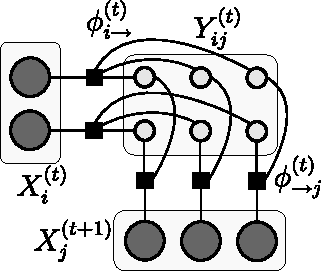
\includegraphics[width=\textwidth]{images/chaingraph/fig_crf_less_nodes.pdf}
        %\rule{\textwidth}{0.3pt}
        \caption{Factor graph representation of the conditional random field at time steps $t$ and
            $t+1$, \ie the undirected part of the chain graph. The assignment variables (smaller,
            light nodes) $Y_{ij}^{(t)}$ are conditioned on the detection variables
            $X_i^{(t)},X_i^{(t+1)}$(dark nodes).}
        \label{fig:chaingraph-crf}
    \end{subfigure}
    \hfill
    \begin{subfigure}[t]{0.48\textwidth}
        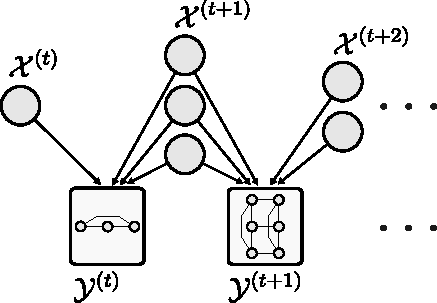
\includegraphics[width=\textwidth]{images/chaingraph/fig_chain_graph.pdf}
        %\rule{\textwidth}{0.3pt}
        \caption{In the directed part of the chain graph the conditional random fields from
            \cref{fig:chaingraph-crf} are subsumed in supernodes (boxes).}
        \label{fig:chaingraph-bn}
    \end{subfigure}
    \caption[Chain graph model]{Conditional random field representation for two consecutive time steps
        of the ``transition model'' (\subref{fig:chaingraph-crf}) and chain graph model for three
        subsequent time steps (\subref{fig:chaingraph-bn}), taken from \citet{kausler_12_discrete}.}
    \label{fig:chaingraph-model}
\end{figure}

After the recap of the chain graph tracking and the conservation tracking factor graph in
\cref{subsec:fg-chaingraph,subsec:fg-conservation}, respectively, we continue with the introduction
of cell identity reconstruction for conservation tracking~(\cref{cha:GMM}) and a new
tracking-by-assignment method, joint segmentation and tracking~(\cref{cha:joint}), which both
address the problem of undersegmentation in cell tracking.


%%% Local Variables: 
%%% mode: latex
%%% TeX-master: "../../../main"
%%% End: 
